\pdfoutput=1
\documentclass[a4paper,pdflatex,ja=standard]{bxjsarticle}

% ---Setting about the geometry of the document----
% \usepackage{a4wide}
% \pagestyle{empty}

% ---Physics and Math Packages---
\usepackage{amssymb,amsfonts,amsthm,mathtools}
\usepackage{physics,braket,bm}

% ---underline---
\usepackage{ulem}

% --- sorround the texts or equations
% \usepackage{fancybox,ascmac}

% ---settings of theorem environment---
% \usepackage{amsthm}
% \theoremstyle{definition}

% ---settings of proof environment---
% \renewcommand{\proofname}{\uline{\textbf{証明}}}
% \renewcommand{\qedsymbol}{$\blacksquare$}

% ---Ignore the Warnings---
\usepackage{silence}
\WarningFilter{latexfont}{Some font shapes,Font shape}

% ---Insert the figure (If insert the `draft' at the option, the process becomes faster)---
\usepackage{graphicx}
% \usepackage{subcaption}

% ----Add a link to a text---
\usepackage{url}
\usepackage{xcolor,hyperref}
\hypersetup{colorlinks=true,citecolor=orange,linkcolor=blue,urlcolor=magenta}
\usepackage{bxcjkjatype}

% ---Tikz---
\usepackage{tikz,pgf,pgfplots,circuitikz}
\pgfplotsset{compat=1.15}
\usetikzlibrary{intersections,arrows.meta,angles,calc,3d,decorations.pathmorphing}

% ---Add the section number to the equation, figure, and table number---
\makeatletter
   \renewcommand{\theequation}{\thesubsection.\arabic{equation}}
   \@addtoreset{equation}{subsection}
   
   \renewcommand{\thefigure}{\thesection.\arabic{figure}}
   \@addtoreset{figure}{section}
   
   \renewcommand{\thetable}{\thesection.\arabic{table}}
   \@addtoreset{table}{section}
\makeatother

% ---enumerate---
\renewcommand{\labelenumi}{\arabic{enumi}.}
\renewcommand{\labelenumii}{(\roman{enumii})}
\renewcommand{\labelenumiii}{(\alph{enumiii})}

% ---Index---
% \usepackage{makeidx}
% \makeindex

% ---Fonts---
\renewcommand{\familydefault}{\sfdefault}

% ---Title---
\title{東京大学\ 平成26年\ 物理学専攻\ 院試\ 解答例}
\author{ミヤネ}
\date{最終更新:\today}

\newcommand{\prb}[2]{
  \phantomsection
  \addcontentsline{toc}{subsection}{問題 #1: #2}
  \subsection*{第#1問\phantom{#2}}
  \setcounter{subsection}{#1}
  \setcounter{equation}{0}
}

\begin{document}

\maketitle

\tableofcontents
\clearpage


\section{数学パート}

\prb{1}{微積分}

\begin{enumerate}

  \item 

  一般解は$y=C_1 e^{-\alpha x}$なので,初期条件より$C_1=Ae^{\alpha b}$となり
  \begin{equation}
    y(x)
    =
    Ae^{-\alpha(x-b)}
  \end{equation}
  です.


  \item 

  第1式より
  \begin{equation}
    y_1(x)
    =
    Ae^{-\alpha x}>0
  \end{equation}
  です.したがって,第2式は
  \begin{equation}
    \dv{y_2(x)}{x}
    +
    \gamma y_2(x)
    =
    A\beta e^{-\alpha x}
  \end{equation}
  となります.この方程式の斉次解は$C_2e^{-\gamma x}$であり,特解は$y_s(x)\equiv C_3e^{-\alpha x}$を代入して
  \begin{equation}
    -
    \alpha C_3
    +
    \gamma C_3
    =
    A\beta
    \quad
    \rightarrow
    \quad
    C_3
    =
    \frac{A\beta}{-\alpha+\gamma}
  \end{equation}
  となるため,一般解は
  \begin{equation}
    y_2(x)
    =
    C_2 e^{-\gamma x}
    +    
    \frac{A\beta}{-\alpha+\gamma}
    e^{-\alpha x}
  \end{equation}
  です.初期条件より$C_2=A\beta/(\alpha-\gamma)$と求まるので,
  \begin{equation}
    y_2(x)
    =
    \frac{A\beta}{\alpha-\gamma}
    (e^{-\gamma x}-e^{-\alpha x})
  \end{equation}
  です.$y_2(x)$の符号は$\alpha,\gamma$の大小関係によらず,
  \begin{equation}
    \left\{
      \begin{alignedat}{1}
        &
        x>0\text{\ のとき,}
        y_2>0
        \\
        &
        x<0\text{\ のとき,}
        y_2<0
      \end{alignedat}
    \right.
    \label{ans12}
  \end{equation}
  です\footnote{
    例えば$\alpha>\gamma$のときを考えます.$\alpha-\gamma>0$なので,$e^{-\gamma x}-e^{-\alpha x}$の符号を考えればよいです.このときは,$x>0$なら$e^{-\gamma x}>e^{-\alpha x}$なので,$y_2>0$で,$x<0$のときは符号がひっくり返ります.$\alpha<\gamma$のときは$\alpha-\gamma<0$なので,$y_2$の符号と$e^{-\gamma x}-e^{-\alpha x}$の符号が反対になります.また,$e^{-\gamma x}-e^{-\alpha x}$の符号も逆転するので,結局\eqref{ans12}になります.
  }.


  \item 

  線形微分方程式なので
  \begin{equation}
    \dv{}{x}
    \begin{pmatrix}
      y_1 \\
      y_2
    \end{pmatrix}
    =
    c
    \begin{pmatrix}
      -1 & \sqrt{3} \\
      \sqrt{3}  & -3  \\
    \end{pmatrix}
    \begin{pmatrix}
      y_1 \\
      y_2
    \end{pmatrix}
    \label{diffeq}
  \end{equation}
  の係数行列の固有値を求めます.計算すれば,固有値と固有ベクトルは
  \begin{equation}
    \lambda_1=-4\ 
    \text{に対して}\ 
    v_1
    =
    \begin{pmatrix}
      1 \\
      -\sqrt{3} 
    \end{pmatrix}
    ,\ 
    \lambda_2=0\ 
    \text{に対して}\ 
    v_2
    =
    \begin{pmatrix}
      \sqrt{3} \\
      1 
    \end{pmatrix}
  \end{equation}
  となるので,対角化すると
  \begin{equation}
    \begin{pmatrix}
      -4 & 0 \\
      0 & 0
    \end{pmatrix}
    =
    P^{-1}
    \begin{pmatrix}
      -1 & \sqrt{3} \\
      \sqrt{3}  & -3  \\
    \end{pmatrix}
    P
    ,\ 
    P
    =
    \begin{pmatrix}
      1 & \sqrt{3} \\
      -\sqrt{3} & 1
    \end{pmatrix}
  \end{equation}
  です.したがって,\eqref{diffeq}に左から$P^{-1}$を作用させ
  \begin{equation}
    \begin{pmatrix}
      Y_1 \\
      Y_2
    \end{pmatrix}
    =
    P^{-1}
    \begin{pmatrix}
      y_1 \\
      y_2
    \end{pmatrix}
    \label{def_Y1Y2}
  \end{equation}
  とおけば
  \begin{equation}
    \dv{}{t}
    \begin{pmatrix}
      Y_1 \\
      Y_2
    \end{pmatrix}
    =
    \begin{pmatrix}
      4cY_1 \\
      0
    \end{pmatrix}
    \quad
    \rightarrow
    \quad
    \begin{pmatrix}
      Y_1 \\
      Y_2 
    \end{pmatrix}
    =
    \begin{pmatrix}
      C_4 e^{-4cx} \\
      C_5
    \end{pmatrix}
  \end{equation}
  と解けます.あとは,$x=0$として\eqref{def_Y1Y2}を代入すれば
  \begin{equation}
    \begin{pmatrix}
      C_4 \\
      C_5
    \end{pmatrix}
    =
    \frac{1}{4}
    \begin{pmatrix}
      1 & -\sqrt{3} \\
      \sqrt{3} & 1
    \end{pmatrix}
    \begin{pmatrix}
      (\sqrt{3}-1)/2 \\
      (\sqrt{3}+1)/2
    \end{pmatrix}
    =
    \frac{1}{2}
    \begin{pmatrix}
      -1  \\
      1
    \end{pmatrix}
  \end{equation}
  となるので,求める解は\eqref{def_Y1Y2}を逆に解いて
  \begin{equation}
    \begin{pmatrix}
      y_1(x) \\
      y_2(x)
    \end{pmatrix}
    =
    \begin{pmatrix}
      1 & \sqrt{3} \\
      -\sqrt{3} & 1
    \end{pmatrix}
    \begin{pmatrix}
      -e^{-4cx}/2 \\
      1/2
    \end{pmatrix}    
    =
    \begin{pmatrix}
      -\dfrac{1}{2}e^{-4cx}
      +
      \dfrac{\sqrt{3}}{2}
      \\
      \dfrac{\sqrt{3}}{2}e^{-4cx}
      +
      \dfrac{1}{2}
    \end{pmatrix}
  \end{equation}
  となります.


  \item 

  $2a$周期の関数なので,フーリエ級数展開
  \begin{equation}
    y(x,t)
    =
    \sum_{n=-\infty}^{\infty}
    \tilde{y}_n(t)e^{-\frac{in\pi}{a}x}
  \end{equation}
  を代入しましょう.ただし,
  \begin{equation}
    \tilde{y}_n(t)
    \equiv
    \frac{1}{2a}\int_{-a}^{a}
    y(x,t)e^{-\frac{in\pi}{a}x}
    \dd x
  \end{equation}
  です.微分方程式を$\tilde{y}_n$についての微分方程式に書き直せば
  \begin{equation}
    \pdv{\tilde{y}_n(t)}{t}
    =
    -
    \left( \frac{n\pi}{a} \right)^2
    t
  \end{equation}
  となるので
  \begin{equation}
    \tilde{y}_{n}(t)
    =
    C^{(n)}
    \exp
    \left[  
      -
      \left( \frac{n\pi}{a} \right)^2
      t
    \right]
  \end{equation}
  と解けます.よって,
  \begin{equation}
    y(t)
    =
    \sum_{n=-\infty}^{\infty}
    A_n \exp
    \left[  
      -
      \left(  
        \frac{n\pi}{a}
      \right)^2
      t
      -
      \frac{in\pi}{a}
      x
    \right]
  \end{equation}
  が一般解です.境界条件を代入すると
  \begin{equation}
    \sum_{n=-\infty}^{\infty}
    A_n (-1)^n \exp
    \left[  
      -
      \left(  
        \frac{n\pi}{a}
      \right)^2
      t
    \right]
    =
    0
  \end{equation}
  となるので,$A_{-n}=-A_n$です.今回は,解を1つでも提示できればよいので,
  \begin{equation}
    A_{n}
    =
    \left\{
      \begin{alignedat}{1}
        1\ &\ (n=1) \\
        -1\ &\ (n=-1) \\
        0\ &\ (\text{それ以外})        
      \end{alignedat}
    \right.
  \end{equation}
  としましょう.すると,微分方程式の解の1つは
  \begin{equation}
    y(x,t)
    =
    -2i
    \sin\left( \frac{\pi}{a}x \right)
    e^{-(\pi/a)^2t}
  \end{equation}
  です.


  \item 

  両辺を$(1-\beta y)y$で割ると
  \begin{equation}
    \left(  
      \frac{\beta}{1-\beta y}
      +
      \frac{1}{y}
    \right)
    \dv{y}{x}
    =
    -\alpha
  \end{equation}
  なので,両辺を$x$で積分すると
  \begin{equation}
    -
    \log(1-\beta y)
    +
    \log y
    =
    -\alpha x+C_6^{*}
  \end{equation}
  となり,
  \begin{equation}
    y(x)
    =
    \frac{C_6 e^{-\alpha x}}{\beta C_6 e^{-\alpha x}+1}
  \end{equation}
  です.ただし,$C_6\equiv e^{C_6}$は積分定数です.初期条件を解けば$C_6$が求まるので
  \begin{equation}
    y(x)
    =
    \frac{Ae^{-\alpha x}}{\beta Ae^{-\alpha x}+1-\beta A}
  \end{equation}
  となります.

\end{enumerate}


\clearpage

\prb{2}{線形代数}

\begin{enumerate}

  \item 

  \begin{enumerate}
    
    \item 

    \begin{equation}
      P
      =
      \begin{pmatrix}
        0 & 1 &   &   &   &     \\
          & 0 & 1 &   &   &     \\
          &   & \ddots &  \ddots  &  &     \\
          &   &        &  \ddots  & \ddots &    \\
          &   &        &          &      0 & 1  \\        
        1 &   &        &          &       & 0 \\
      \end{pmatrix}
      .
    \end{equation}


    \item 

    $PA$を計算すると
    \begin{align}
      PA
      &=
      \begin{pmatrix}
        0 & 1 &   &   &   &     \\
          & 0 & 1 &   &   &     \\
          &   & \ddots &  \ddots  &  &     \\
          &   &        &  \ddots  & \ddots &    \\
          &   &        &          &      0 & 1  \\        
        1 &   &        &          &       & 0 \\
      \end{pmatrix}
      \begin{pmatrix}
        \varepsilon & t &   &   &   &   t  \\
        t & \varepsilon & t &   &   &     \\
          &  \ddots & \ddots &  \ddots  &  &     \\
          &   &    \ddots   &  \ddots  & \ddots &    \\
          &   &        &     t     &      \varepsilon & t  \\        
        t &   &        &          &    t   & \varepsilon \\
      \end{pmatrix}
      \nonumber
      \\
      &=
      \begin{pmatrix}
        t & \varepsilon & t  &   &   &     \\
          & t & \varepsilon & t  &   &     \\
          &   & \ddots &  \ddots  &\ddots  &     \\
          &   &        &  \ddots  & \ddots & t  \\
        t  &   &        &          &      t & \varepsilon  \\        
        \varepsilon & t  &        &          &       & t \\
      \end{pmatrix}
    \end{align}
    となりますが,$AP$を計算すると
    \begin{equation}
      AP
      =
      \begin{pmatrix}
        t & \varepsilon & t  &   &   &     \\
          & t & \varepsilon & t  &   &     \\
          &   & \ddots &  \ddots  &\ddots  &     \\
          &   &        &  \ddots  & \ddots & t  \\
        t  &   &        &          &      t & \varepsilon  \\        
        \varepsilon & t  &        &          &       & t \\
      \end{pmatrix}
    \end{equation}
    と全く同じ結果になります.よって,$PA-AP=0$です.


    \item 

    固有方程式は
    \begin{equation}
      \begin{vmatrix}
        \lambda & -1 &   &   &   &     \\
          & \lambda & -1 &   &   &     \\
          &   & \ddots &  \ddots  &  &     \\
          &   &        &  \ddots  & \ddots &    \\
          &   &        &          & \lambda & -1  \\        
        -1 &   &        &          &       & \lambda \\
      \end{vmatrix}
      =
      0
    \end{equation}
    です.余因子展開を用いると
    \begin{equation}
      \begin{vmatrix}
        \lambda & -1 &   &   &   &     \\
          & \lambda & -1 &   &   &     \\
          &   & \ddots &  \ddots  &  &     \\
          &   &        &  \ddots  & \ddots &    \\
          &   &        &          & \lambda & -1  \\        
        -1 &   &        &          &       & \lambda \\
      \end{vmatrix}
      =
      \lambda
      \begin{vmatrix}
        \lambda & -1 &   &   &   &     \\
          & \lambda & -1 &   &   &     \\
          &   & \ddots &  \ddots  &  &     \\
          &   &        &  \ddots  & \ddots &    \\
          &   &        &          & \lambda & -1  \\        
          &   &        &          &       & \lambda \\
      \end{vmatrix}    
      +
      \begin{vmatrix}
        0 & -1 &   &   &      \\
          & \lambda & -1 &   &        \\
          &   & \ddots &  \ddots  &       \\
          &   &        &  \ddots  & -1 \\
          &   &        &          & \lambda   \\       
      \end{vmatrix}
    \end{equation}
    となりますが,第1項は上三角行列なので対角項の積でになり,第2項は余因子展開を繰り返すと
    \begin{equation}    
      \begin{vmatrix}
        0 & -1 &   &   &   &     \\
          & \lambda & -1 &   &   &     \\
          &   & \ddots &  \ddots  &  &     \\
          &   &        &  \ddots  & \ddots &    \\
          &   &        &          & \lambda & -1  \\        
        -1 &   &        &          &       & \lambda \\
      \end{vmatrix}
      =
      \cdots
      =
      \begin{vmatrix}
        0 & -1 & 0 \\
        0 & \lambda & -1 \\
        -1 & 0 & \lambda
      \end{vmatrix}
      =
      -1
    \end{equation}
    となるので\footnote{
      余因子展開で$(1,2)$成分を展開するときに$-1$が出てきますが,その成分が$-1$なので,符号を変えずに$1$行$2$列を削って行くことができます.
    }
    \begin{equation}
      \lambda^n
      =
      1
    \end{equation}
    が固有方程式です\footnote{
      余談ですが,最初に解いたとき,$3\times 3$行列と同じように行列式を計算してしまったため,固有方程式が
      $$
        \lambda^n
        +
        (-1)^n
        =
        0
      $$
      となってしまい,かなり痛い目を見ました.気をつけたいです.
    }\footnote{
      ちなみに,この行列についてはもっと技巧的な固有値の求め方があります.ここでは紹介しませんが,「3重対角行列」などが参考になるかと思います.ここでは,ゴリゴリ計算しました.
    }.これを解くと,求める固有値は
    \begin{equation}
      \lambda_k
      =
      e^{2\pi i k/n}
      \quad
      (k=1,\cdots,n)
    \end{equation}
    となります.固有ベクトルは,連立方程式
    \begin{equation}    
      \begin{pmatrix}
        \lambda_k & -1 &   &   &   &     \\
          & \lambda_k & -1 &   &   &     \\
          &   & \ddots &  \ddots  &  &     \\
          &   &        &  \ddots  & \ddots &    \\
          &   &        &          & \lambda_k & -1  \\        
        -1 &   &        &          &       & \lambda_k \\
      \end{pmatrix}
      \begin{pmatrix}
        x_1 \\
        x_2 \\
        \vdots \\
        \vdots \\
        x_{n-1} \\
        x_n
      \end{pmatrix}
      =
      0
    \end{equation}
    を解くことになりますが,$x_1=1$とおけば,固有値$\lambda_k$に対応する固有ベクトル$\bm{u}_k$は
    \begin{equation}
      \bm{u}_k
      =
      \begin{pmatrix}
        1 \\
        \lambda_k \\
        \vdots \\
        \vdots \\
        \lambda_k^{n-2} \\
        \lambda_k^{n-1}
      \end{pmatrix}
    \end{equation}
    です.


    \item 

    $A=t(P+P^{T})+\varepsilon I$と展開できます.$P^{T}$を$\bm{u}_k$に作用させてみると
    \begin{equation}    
      \begin{pmatrix}
        0 &  &   &   &   &   1  \\
        1  & 0 &  &   &   &     \\
          &  \ddots   & \ddots &  &  &     \\
          &   &     \ddots    &  \ddots  & &    \\
          &   &        &      1    &      0 &   \\        
          &   &        &          &   1    & 0 \\
      \end{pmatrix}
      \begin{pmatrix}
        1 \\
        \lambda_k \\
        \vdots \\
        \vdots \\
        \lambda_k^{n-2} \\
        \lambda_k^{n-1}
      \end{pmatrix}
      =
      \begin{pmatrix}
        \lambda_k^{n-1} \\
        1 \\
        \lambda_k \\
        \vdots \\
        \vdots \\
        \lambda_k^{n-2}
      \end{pmatrix}
      =
      \frac{1}{\lambda_k}
      \bm{u}_k
    \end{equation}
    となるので,固有値$1/\lambda_k$の固有ベクトルとなってます.したがって,
    \begin{equation}
      A\bm{u}_k
      =
      \left[  
        t\left( e^{2\pi ik/n}+e^{-2\pi ik/n} \right)
        +
        \varepsilon
      \right]
      \bm{u}_k
      =
      (2t\cos(2\pi k/n)+\varepsilon)
      \bm{u}_k
    \end{equation}
    です.$\bm{u}_k$は$A$の固有ベクトルであり,$k\neq l$なら固有値が異なります.$A$はエルミートなので,$\bm{x},\bm{y}$の固有値を$x,y$とおけばこれらは実数で
    \begin{equation}
      \bm{x}^{\dag}A\bm{y}
      =
      x
      \bm{x}^{\dag}\bm{y}
      =
      y
      \bm{x}^{\dag}\bm{y}
      \quad
      \rightarrow
      \quad
      (x-y)
      \bm{x}^{\dag}\bm{y}
      =
      0
    \end{equation}
    となります.よって,$x\neq y$なので,$\bm{x}^{\dag}\bm{y}=0$で$\bm{x}^{\dag}A\bm{y}=0$です.


    \item 

    $U$を
    \begin{equation}
      U
      =
      \frac{1}{\sqrt{n}}
      \begin{pmatrix}
        \bm{u}_1
        &
        \cdots
        &
        \bm{u}_n
      \end{pmatrix}
    \end{equation}
    とおけば,$\bm{u}_k^{\dag}\bm{u}_l=n\delta_{kl}$なので$U$はユニタリーになります($\sqrt{n}$で規格化しておくのが重要).$D$の$\bm{u}_k$に対する固有値は分かっているので
    \begin{equation}
      D
      =
      \begin{pmatrix}
        2t\cos(2\pi/n)+\varepsilon & & &  & \\
          &2t\cos(4\pi/n)+\varepsilon& & & & \\
          &                          & \ddots & & \\
          & & &2t\cos(2\pi (n-1)/n)+\varepsilon & \\
          & & & & 2t+\varepsilon
      \end{pmatrix}
      \label{D}
    \end{equation}
    です.

  \end{enumerate}

  
  \item 

  \begin{enumerate}

    \item 

    ちゃんと計算すると大変なので,少し工夫しましょう.固有方程式は
    \begin{equation}
      \begin{vmatrix}
        A(0,t)-\Lambda & \lambda I \\
        \lambda I & A(0,2t)-\Lambda
      \end{vmatrix}
      =
      \begin{vmatrix}
        A(-\Lambda,t) & \lambda I \\
        \lambda I & A(-\Lambda,2t)
      \end{vmatrix}
      =
      0
    \end{equation}
    ですが,これに次の$2n$次正方行列
    \begin{equation}
      P
      =
      \begin{pmatrix}
        U & 0 \\
        0 & U
      \end{pmatrix}
    \end{equation}
    を作用させることを考えます.行列$\lambda I-B$を$P$と$P^{-1}$で挟むと
    \begin{align}
      P^{-1}(\lambda I-B)P
      &=
      \begin{pmatrix}
        U^{-1} & 0 \\
        0 & U^{-1}
      \end{pmatrix}
      \begin{pmatrix}
        A(-\Lambda,t) & \lambda I \\
        \lambda I & A(-\Lambda,2t)
      \end{pmatrix}
      \begin{pmatrix}
        U & 0 \\
        0 & U
      \end{pmatrix}
      \nonumber
      \\
      &=
      \Lambda I
      -
      \begin{pmatrix}
        U^{-1}A(-\Lambda,t)U & \lambda I \\
        \lambda I & U^{-1}A(-\Lambda,2t)U
      \end{pmatrix}
    \end{align}
    となりますが,$\det P^{-1}=1/\det P$であることに気をつければ,固有方程式は
    \begin{equation}
      \begin{vmatrix}
        D(-\Lambda,t) & \lambda I \\
        \lambda I & D(-\Lambda,2t)
      \end{vmatrix}
      =
      0
      \label{char_eq1}
    \end{equation}
    と同値であることが分かります.ただし,$D(\varepsilon,t)$は前問の答え\eqref{D}です.行列式を計算するために,基本変形をして上三角行列を作りましょう.そのためには,「第$k$行を$-\lambda/(2t\cos(2\pi k/n)-\Lambda)$倍して第$k+n$行に加え」れば良いです.すると,対角成分は$D(-\Lambda,t)$と,「$(-\Lambda,2t)$の第$l$成分から$\lambda^2/(2t\cos(2\pi k/n)-\Lambda)$を引いたもの」が対角成分に並ぶことになります.よって,固有方程式は
    \begin{equation}
      \prod_{k=1}^{n}
      \left(  
        2t\cos(2\pi k/n)-\Lambda
      \right)
      \prod_{l=1}^{n}
      \left(  
        4t\cos(2\pi l/n)
        -
        \Lambda
        -
        \frac{\lambda^2}{2t\cos(2\pi l/n)-\Lambda}
      \right)
      =
      0
      \label{char_eq2}
    \end{equation}
    となるので,$2n$個の固有値とは
    \begin{equation}
      \Lambda_l
      =
      3t\cos(2\pi l/n)
      \pm
      \sqrt{t^2\cos^2(2\pi l/n)+\lambda^2}
    \end{equation}
    です\footnote{
      \eqref{char_eq2}のうち,基本変形で$\Lambda\neq 2t\cos(2\pi k/n)$を仮定しているため,第1項は解には成りえません.
    }.


    \item 

    $\lambda=0$なら,$\Lambda_l=2t\cos(2\pi l/n),4t\cos(2\pi l/n)$となりますが,これは\eqref{char_eq1}より明らかです.また,$\lambda\ll t$なら,
    \begin{align}
      \Lambda_l
      &=
      3t\cos(2\pi l/n)
      \pm
      t\cos(2\pi l/n)
      \sqrt{
        1+\left( \frac{\lambda}{t\cos(2\pi l/n)} \right)^2
      }
      \nonumber
      \\
      &\sim      
      3t\cos(2\pi l/n)
      \pm
      t\cos(2\pi l/n)
      \pm
      \frac{\lambda^2}{2t\cos(2\pi l/n)}
    \end{align}
    なので,ズレは$\lambda^2$に比例します.

  \end{enumerate}


\end{enumerate}



\clearpage

\section{物理パート}

\prb{1}{量子力学}

\begin{enumerate}

  \item 

  Schrödinger方程式は
  \begin{equation}
    \left[  
      -\frac{\hbar^2}{2m}
      \left(  
        \dv[2]{}{r}
        +
        \frac{2}{r}
        \dv{}{r}
      \right)
      -
      \frac{q^2}{4\pi\varepsilon_0}
      \cdot
      \frac{1}{r}
    \right]
    \psi
    =
    E\psi
  \end{equation}
  なので,$r=r_0\rho,\ E=-E_0\varepsilon$を代入すると
  \begin{equation}
    \left[  
      \dv[2]{}{\rho}
      +
      \frac{2}{\rho}
      \dv{}{\rho}
      +
      \underset{=2}{
        \uwave{
          \frac{2mq^2r_0}{4\pi\varepsilon_0\hbar^2}
        }
      }
      \cdot
      \frac{1}{\rho}
    \right]
    \psi
    =
    \underset{=1}{\uwave{
      \frac{2mE_0r_0^2}{\hbar^2}
      }
    }
    \varepsilon\psi
  \end{equation}
  となり,
  \begin{equation}
    r_0
    =
    \frac{4\pi\hbar^2\varepsilon_0}{mq^2}
    ,\ 
    E_0
    =
    \frac{mq^2}{32\pi^2\varepsilon_0^2\hbar^2}
  \end{equation}
  です.


  \item 

  $\psi=ce^{-\rho}$を微分方程式(1)に代入すると$\varepsilon=1$が分かります.よって
  \begin{equation}
    E
    =
    -E_0
    .
  \end{equation}
  また,$r^2$の期待値は
  \begin{equation}
    \ev*{r^2}
    =
    \int\dd^3\bm{r}\ 
    \psi^{*}(\bm{r})r^2\psi(\bm{r})
    =
    4\pi|c|^2
    \int_0^{\infty}
    r^4 e^{-2r/r_0}
    \dd r
  \end{equation}
  ですが,
  \begin{equation}
    \int_0^{\infty}
    r^4 e^{-2r/r_0}
    \dd r
    =
    \frac{3}{4}r_0^5    
  \end{equation}
  なので
  \begin{equation}
    \ev*{r^2}
    =
    3\pi|c|^2r_0^5
  \end{equation}
  です.ここで,規格化定数は
  \begin{equation}
    4\pi|c|^2\int_{0}^{\infty}
    \psi^*\psi
    \dd r
    =
    \pi|c|^2r_0^3
    =1
    \quad
    \rightarrow
    \quad
    |c|^2
    =
    \frac{1}{\pi r_0^3}
  \end{equation}
  なので,
  \begin{equation}
    \sqrt{\ev*{r^2}}
    =
    \sqrt{3}r_0
  \end{equation}
  です.


  \item
  
  計算するだけです:
  \begin{equation}
    [p_1,p_2]
    =
    -i\hbar qB
    ,\ 
    [p_2,p_z]
    =
    [p_z,p_1]
    =
    0
    .
  \end{equation}


  \item

  $[X,p]=k[p_2,p_1]=i\hbar kqB$なので,$k=1/qB$とおけば$X,P$は正準変数です.また,ハミルトニアンは
  \begin{equation}
    H
    =
    \frac{P^2}{2m}
    +
    \frac{m\omega^2}{2}X^2
    +
    \frac{p_z^2}{2m}
    ,\ 
    \omega
    \equiv
    \frac{qB}{m}
  \end{equation}
  となるので,確かに$(x,y)$方向では調和振動.古典的に考えれば,$\omega$は円運動の周期です.


  \item 

  $P'$が$X,P$と可換なのはよいでしょう.$X'=C_1 x+C_2 p_y$とおいて係数$C_1,C_2$を計算します.$X'$が$X$と交換するのは明らかなので,$P$との交換関係を調べれば
  \begin{equation}
    [X',P]
    =
    i\hbar
    \left(  
      C_1
      +
      \frac{qB}{2}C_2
    \right)
  \end{equation}
  です.$(\cdots)$の中身が1になるように$C_1,C_2$をとればよいので,$C_2=1$とおけば
  \begin{equation}
    X'
    =
    -\frac{qB}{2}x
    +
    p_y
  \end{equation}
  です.


  \item  

  基底状態の$(X,P)$に対する運動方程式は
  \begin{equation}
    -\frac{\hbar^2}{2m}
    \dv[2]{\psi_0(X)}{X}
    +
    \frac{m\omega^2}{2}X^2\psi_0(X)
    =
    0
  \end{equation}
  です.これは級数展開で解けます.$\psi_0$を
  \begin{equation}
    \psi_0(X)
    =
    \sum_{n=0}^{\infty}
    c_n X^n
  \end{equation}
  のように展開すれば,微分方程式は
  \begin{equation}
    \sum_{n=2}^{\infty}
    \left[  
      (n+2)(n+1)c_{n+2}
      -
      \left( \frac{m\omega}{\hbar} \right)^2
      c_{n-2}
    \right]
    X^n
    -
    \left(  
      \frac{m\omega}{\hbar} 
    \right)^2
    \left[  
      c_1 X+c_0
    \right]
  \end{equation}
  です.これを解けば
  \begin{equation}
    c_0=c_1=0
    ,\ 
    c_{n+2}
    =
    \frac{1}{(n+1)(n+2)}
    \left(  
      \frac{m\omega}{\hbar} 
    \right)^2
    c_{n-2}
  \end{equation}
  です\footnote{
    これ以上どうこう言えるような気がしません.微分方程式が間違っている?(or そもそもこの方程式は解き方がある?)
  }.

  また,$X'=a$とおけるとき,設問5の答えをみれば,
  \begin{equation}
    X
    =
    x-\frac{a}{qB}
  \end{equation}
  と変数変換できることが分かります.これはただの平行移動です.$x$が元々の座標ということは,$a$は振動(古典的描像なら円運動)の中心であることが分かります.


\end{enumerate}


\subsection*{補足}

\begin{itemize}

  \item 

  ちなみに,今回のような,背景磁場があるときの粒子の運動の量子化を「ランダウ準位」といいます.古典論から予測できる通り,磁場に垂直な平面の運動は調和振動になります.量子力学Cでやったかは覚えていないですが,あまり主要な教科書には載ってないんじゃないかと思います.(私は素粒子特論Dという授業で知りました.どうやら,ランダウ=リフシッツの本には載っているようです.)


\end{itemize}


\clearpage

\prb{2}{統計力学}

\begin{enumerate}

  \item 

  自由場なので,エネルギーは
  \begin{equation}
    \varepsilon_{\bm{k}}
    =
    \frac{\hbar^2\bm{k}^2}{2m}
    \label{energy}
  \end{equation}
  です\footnote{
    $\psi=e^{i\bm{k}\cdot\bm{r}}$として,Schrödinger方程式に代入します.
  }.したがって,一辺の長さが$L$の正方形に閉じ込められているので,$x$方向の波動関数は
  \begin{equation}
    \psi_n(x)
    =
    \sin\left( \frac{n\pi}{L} x \right)
    ,\ 
    k_n
    =
    \frac{n\pi}{L}
  \end{equation}
  と量子化されます.(ただし規格化はしてません.)これを満たす$(k_x,k_y)$を図示すると,中心から状態が詰まっていくことが分かります.

  \begin{figure}[ht]    
    \centering
    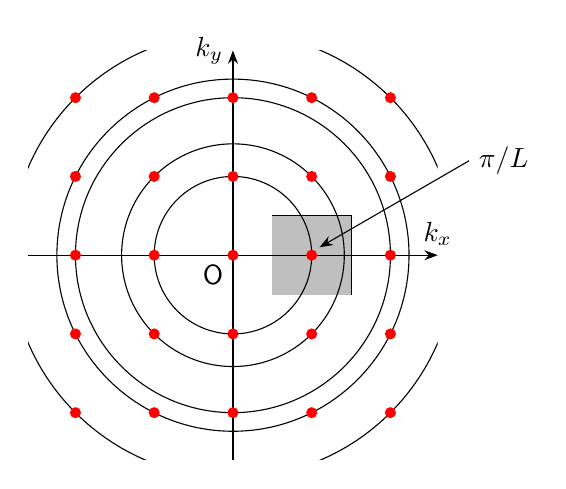
\begin{tikzpicture}
      \draw[thin](0.5,0.5)--(1.5,0.5)--(1.5,-0.5)--(0.5,-0.5)--cycle;
      \fill[lightgray](0.5,0.5)--(1.5,0.5)--(1.5,-0.5)--(0.5,-0.5)--cycle;
      \draw[-Stealth] (-2.6,0)--(2.6,0)node[above]{$k_x$};
      \draw[-Stealth] (0,-2.6)--(0,2.6)node[left]{$k_y$};      
      \begin{scope} \clip (-2.6,-2.6) rectangle (2.6,2.6);
        \draw(0,0) circle (1);
        \draw(0,0) circle ({sqrt(2)});
        \draw(0,0) circle (2);      
        \draw(0,0) circle ({sqrt(5)}); 
        \draw(0,0) circle ({2*sqrt(2)});       
        \fill[red](0,0) circle (2pt);     
        \draw(0,0)node[below left]{O};
        \fill[red](1,0) circle (2pt);
        \fill[red](1,1) circle (2pt);\fill[red](1,2) circle (2pt);\fill[red](2,0) circle (2pt);\fill[red](2,1) circle (2pt);\fill[red](2,2) circle (2pt);\fill[red](1,-1) circle (2pt);\fill[red](1,-2) circle (2pt);\fill[red](2,-1) circle (2pt);\fill[red](2,-2) circle (2pt);\fill[red](0,-2) circle (2pt);\fill[red](0,-1) circle (2pt);\fill[red](0,1) circle (2pt);\fill[red](0,2) circle (2pt);\fill[red](-1,0) circle (2pt);\fill[red](-1,1) circle (2pt);\fill[red](-1,2) circle (2pt);\fill[red](-2,0) circle (2pt);\fill[red](-2,1) circle (2pt);\fill[red](-2,2) circle (2pt);\fill[red](-1,-1) circle (2pt);\fill[red](-1,-2) circle (2pt);\fill[red](-2,-1) circle (2pt);\fill[red](-2,-2) circle (2pt);
      \end{scope}
      \draw[-Stealth] (3,1.2)--(1.1,0.1);
      \draw(3,1.2)node[right]{$\pi/L$};
    \end{tikzpicture}   
    \caption{$(k_x,k_y)$の取りうる値}
    \label{kxky_plane}
  \end{figure}

  図\ref{kxky_plane}の灰色部分の面積は$\pi^2/L^2$ですが,この$(k_x,k_y)$平面では$\pi^2/L^2$あたり1つの格子点があることになります.したがって,$N_0$個の点が存在するとき,$\pi^2 N_0/L^2$の面積を占めることになります.半径を$k\equiv|\bm{k}|$とおけば
  \begin{equation}
    \pi k^2
    =
    \frac{\pi^2}{L^2}N_0
  \end{equation}
  と近似できるので,このときのエネルギーは
  \begin{equation}
    \varepsilon
    =
    \frac{\hbar^2}{2m}
    \cdot
    \frac{\pi}{L^2}N_0    
    =
    \frac{\pi\hbar^2 N_0}{2mL^2}
  \end{equation}
  となります.


  \item 

  $E_N=\sum n_k\varepsilon_k,\ N=\sum n_k$を$\exp$の肩に代入すれば
  \begin{equation}
    e^{-\beta(E_N-\mu N)}
    =
    \exp\left[  
      \sum_{k}[-\beta(\varepsilon_k-\mu)n_k]
    \right]
    =
    \prod_{k}
    e^{-\beta(\varepsilon_k-\mu)n_k}
  \end{equation}
  とできます.したがって,因数分解を行えば
  \begin{equation}
    \Xi[T,\mu]
    =
    \sum_{N=0}^{\infty}
    \left(  
      \prod_{k}
      \sum_{\{n_k\}}
      e^{-\beta(\varepsilon_k-\mu)n_k}
    \right)
  \end{equation}
  と因数分解することができます.$n_k$での和は自由に行うことができませんが\footnote{
    この段階では,まだ,$N=\sum n_k$の制約があります.
  },$N$が自由に動くことを考慮すれば因数分解を同様に行うことで
  \begin{equation}
    \Xi[T,\mu]
    =
    \prod_{k=0}^{\infty}
    \left(  
      \sum_{n_k=0}^{\infty}
      e^{-\beta(\varepsilon_k-\mu)n_k}
    \right)
    =
    \left(  
      \sum_{n_0=0}^{\infty}
      e^{-\beta(\varepsilon_0-\mu)n_0}      
    \right)
    \left(  
      \sum_{n_1=0}^{\infty}
      e^{-\beta(\varepsilon_1-\mu)n_1}      
    \right)
    \cdots
  \end{equation}
  と,各準位に分解することができます.


  \item 

  フェルミ粒子を考えているので,各準位に対して粒子は1つしか入ることができません.つまり$n_k$が取りうる値は0と1だけなので  
  \begin{equation}    
    \Xi_k[T,\mu]
    \equiv
    \sum_{n_k=0}^{\infty}
    e^{-\beta(\varepsilon_k-\mu)n_k}
    =
    1
    +
    e^{-\beta(\varepsilon_k-\mu)}
  \end{equation}
  です.定義から,第$k$準位にある粒子の平均$\bar{n}_k$は
  \begin{equation}
    \bar{n}_k
    =
    \frac{1}{\beta}\pdv{}{\mu}\log\Xi_k[T,\mu]
    =
    \frac{1}{e^{\beta(\varepsilon_k-\mu)}+1}
    =
    f(\varepsilon_k)
  \end{equation}
  となります.一方で,
  \begin{equation}
    \Xi[T,\mu]
    =
    \Xi_0[T,\mu]
    \times
    \Xi_1[T,\mu]
    \times
    \cdots
    =
    \prod_{k=0}^{\infty}
    \Xi_k[T,\mu]
  \end{equation}
  なので,
  \begin{equation}
    \overline{N}
    =
    \frac{1}{\beta}\pdv{}{\mu}\log\Xi[T,\mu]
    =
    \sum_{k=0}^{\infty}
    \left(  
      \frac{1}{\beta}\pdv{}{\mu}\log\Xi_k[T,\mu]
    \right)
    =
    \sum_{k=0}^{\infty}
    \bar{n}_k
  \end{equation}
  です.よって,式(2)が示されました.

  また,和を積分に直すとき,
  \begin{equation}
    \overline{N}
    =
    \sum_{n=0}^{\infty}
    \frac{1}{e^{\beta(\varepsilon_n-\mu)}+1}
    =
    \frac{1}{\Delta k_x\Delta k_y}
    \sum_{n=0}^{\infty}
    \frac{\Delta k_x\Delta k_y}{e^{\beta(\varepsilon_n-\mu)}+1}
  \end{equation}
  となるはずです.ここで,$\Delta k$は$k_n=n\pi/L$より$\pi/L$です.よって,
  \begin{equation}
    \overline{N}
    \sim
    \frac{L^2}{\pi^2}
    \int\dd \bm{k}\     
    \frac{1}{e^{\beta(\varepsilon_{\bm{k}}-\mu)}+1}
    \label{ave_num_part}
  \end{equation}
  となります.ただし,$\varepsilon_{\bm{k}}$は\eqref{energy}です.この積分は極座標で行うと便利で
  \begin{align}
    \int\dd \bm{k}\     
    \frac{1}{e^{\beta(\varepsilon_{\bm{k}}-\mu)}+1}
    &=
    \int_{0}^{2\pi}\dd \theta\int_{0}^{\infty}k\dd k\     
    \frac{1}{e^{\beta(\hbar^2 k^2/2m-\mu)}+1}
    \nonumber
    \\
    &=
    \frac{m}{\hbar^2}
    \int_{0}^{\infty}
    \frac{\dd \varepsilon}{e^{\beta(\varepsilon-\mu)}+1}
    \qquad
    \left(  
      \because
      \ 
      \dd \varepsilon
      =
      \frac{m}{\hbar^2}
      k\dd k
    \right)
    \nonumber
    \\
    &=
    \frac{\beta m}{\hbar^2}
    \int_{e^{-\beta\mu}}^{\infty}
    \frac{\dd z}{z(z+1)}
    \qquad
    \left(  
      z\equiv e^{\beta(\varepsilon-\mu)}
      \text{と変数変換}
    \right)
    \nonumber
    \\  
    &=
    \frac{m}{\hbar^2}
    \left[  
      \beta\mu
      +
      \log(1+e^{-\beta\mu})
    \right]
  \end{align}
  となります.


  \item 
  
  \begin{figure}[ht]
    \centering    
    \begin{tikzpicture}[scale=2.0]  
        \draw[->,>=stealth,ultra thin](-0.5,0)--(2,0)node[below]{$\varepsilon$};
        \draw[->,>=stealth,thin](0,-0.5)--(0,1.5)node[right]{$f(\varepsilon)$};
        \draw[dashed,ultra thin](-0.5,1)--(2,1);
        \draw[dotted,thin](1,1/2)--(1,0)node[below]{$\mu$};
        \draw[dotted,thin](1,1/2)--(0,1/2)node[left]{$1/2$};
        \draw(0,0)node[below left]{O};
        \draw(0,1)node[above left]{$1$};
        \draw[thin,samples=100,domain=-0.5:2]plot(\x,{1/(exp(1.2*(\x-1))+1)})node[right]{高温};    
        \draw[thick,samples=100,domain=1.8:-0.5]plot(\x,{1/(exp(10*(\x-1))+1)})node[left]{低温};    
      \end{tikzpicture}   
    \caption{$f(\varepsilon)$の概略図}
    \label{fermi_dist}
  \end{figure}

  $f(\varepsilon)$の概形は図\ref{fermi_dist}の通りです.$T$が増加すると$\varepsilon=\mu$付近で粒子数が増加しますが,その増加量は 
  \begin{equation}
    \pdv{f}{T}
    =
    -
    \frac{\varepsilon-\mu}{k_BT^2}
    \cdot
    \frac{e^{(\varepsilon-\mu)/k_BT}}{\left( e^{(\varepsilon-\mu)/k_BT}+1 \right)^2}
    =
    -
    \frac{\varepsilon-\mu}{4k_BT^2}
    \cdot
    \frac{1}{\cosh^2\left( \frac{\varepsilon-\mu}{2k_BT} \right)}
  \end{equation}
  と書けます.ここで,$\varepsilon\sim\mu$付近では,$\cosh x\sim 1-x^2/2$なので
  \begin{equation}
    \left.
      \pdv{f}{T}
    \right|_{\varepsilon\sim\mu}
    \propto
    T^2
  \end{equation}
  です.したがって,$\varepsilon$よりもエネルギーが大きい粒子は$T\sim0$では$T^2$で増えることになり,それに伴ってエネルギーも$T^2$で増加し,よって,比熱は$T$に比例することになります.


  \item

  基本的には$\varepsilon<0$の領域に粒子が詰まって行きますが,取りうる状態の数が増えてくると$\varepsilon\sim -\Delta$付近の粒子が$\varepsilon\sim+\Delta$に励起されます\footnote{
    詳しい議論は「フェルミ縮退」を参考にするとよいでしょう.たぶん.もしくは,次の設問も参考になるかもしれません.
  }.


  \item

  今回の状況では,\eqref{ave_num_part}より
  \begin{equation}
    \overline{N}_1(T)
    =
    \overline{N}_1(0)
    -
    \frac{L^2}{\pi^2}
    \int_{0}^{\infty}\dd \bm{k}\     
    \frac{1}{e^{\beta(\varepsilon_{\bm{k}}-\mu)}+1}
  \end{equation}
  が成立しています\footnote{
    $\overline{N}_1(T)$は「負のエネルギーの粒子数」ですが,それは「$T=0$で$\varepsilon<0$に存在した粒子数」から「温度が$T$上昇したことで$\varepsilon>0$に遷移した粒子数」を引くことで求めることができるはずです.温度$T$における粒子数は,設問3で求めているので,それを用いれば$\mu$について解けそうです.
  }.ここで,低温$\beta\mu\gg 1$なので,この関係式は
  \begin{equation}
    \mu
    \sim 
    \frac{\hbar^2 k_BT}{m}
    \left[  
      \overline{N}_1(0)
      -
      \overline{N}_1(T)
    \right]
  \end{equation}
  と解けます.


\end{enumerate}


\clearpage

\prb{3}{電磁気学}

\begin{enumerate}

  \item 

  式(3)より,磁場$\bm{H}$は
  \begin{equation}
    \bm{H}
    =
    \frac{k}{\mu_0\omega}(\bm{e}_z\times\bm{E}_0)
    e^{i(kz-\omega t)}
    \label{mag_field}
  \end{equation}
  であり,式(4)で$\bm{j}=0$としたものに$\bm{H}$と$\bm{E}$の表式を代入すると
  \begin{equation}
    \frac{k^2}{\mu_0\omega}\bm{E}_0
    =
    \omega\varepsilon_{\mathrm{d}}\bm{E}_0
  \end{equation}
  となり\footnote{
    ただし,$\bm{e}_z\cdot\bm{E}=0$としました.
  },
  \begin{equation}
    \frac{k}{\omega}
    =
    \sqrt{\varepsilon_{\mathrm{d}}\mu_0}
  \end{equation}
  です.また,位相速度は
  \begin{equation}
    v_{\mathrm{p}}
    \equiv
    \frac{\omega}{k}
    =
    \frac{1}{\sqrt{\varepsilon_{\mathrm{d}}\mu_0}}
  \end{equation}
  です.


  \item

  式(3)の$\mathrm{rot}$をとると
  \begin{equation}
    -
    \nabla^2\bm{E}
    =
    -\mu_0\pdv{\bm{j}}{t}
    -\varepsilon_{\mathrm{m}}\mu_0\pdv[2]{\bm{E}}{t}
  \end{equation}
  となるので
  \begin{equation}
    \left(  
      \nabla^2
      -
      \mu_0\sigma
      \pdv{}{t}
      -
      \varepsilon_{\mathrm{m}}\mu_0\pdv[2]{}{t}      
    \right)
    \bm{E}
    =
    0
    \label{diffeq_E}
  \end{equation}
  です.


  \item

  式(3),(4)からは,接線方向の接続条件が出てきます.したがって,境界面をまたぐような経路をとって,式(3)を面積分すれば
  \begin{equation}
    \int_{S}
    (\bm{\nabla}\times\bm{E})
    \cdot
    \dd \bm{S}
    =
    -\pdv{}{t}
    \int_S
    \bm{B}
    \cdot
    \dd \bm{S}
  \end{equation}
  となります.経路の厚さを0にすると,右辺の面積分は0.左辺はストークスの定理に直せて,接線方向のみが残り
  \begin{equation}
    \bm{E}_{\mathrm{i}0}
    +
    \bm{E}_{\mathrm{r}0}
    =
    \bm{E}_{\mathrm{m}0}
    \label{bound_E}
  \end{equation}
  です.同様に,界面に電流が流れていないとすれば,式(4)は
  \begin{equation}
    \bm{H}_{\mathrm{i}0}
    +
    \bm{H}_{\mathrm{r}0}
    =
    \bm{H}_{\mathrm{m}0}
    \label{bound_H}    
  \end{equation}
  となります.ここで,\eqref{mag_field}より
  \begin{equation}
    \left\{
      \begin{alignedat}{1}
        \bm{H}_{\mathrm{i}0}
        &=
        \frac{k}{\mu_0\omega}(\bm{e}_z\times\bm{E}_{\mathrm{i}0})
        e^{i(kz-\omega t)}
        \\
        \bm{H}_{\mathrm{r}0}
        &=
        -
        \frac{k}{\mu_0\omega}(\bm{e}_z\times\bm{E}_{\mathrm{r}0})
        e^{i(-kz-\omega t)}
        \\
        \bm{H}_{\mathrm{m}0}        
        &=
        \frac{k_{\mathrm{m}}}{\mu_0\omega}(\bm{e}_z\times\bm{E}_{\mathrm{m}0}  )
        e^{i(k_{\mathrm{m}}z-\omega t)}
      \end{alignedat}
    \right.
  \end{equation}
  なので,\eqref{bound_H}は
  \begin{equation}
    k\bm{E}_{\mathrm{i}0}
    -
    k\bm{E}_{\mathrm{r}0}
    =
    k_{\mathrm{m}}\bm{E}_{\mathrm{m}0}
    \label{bound_E2}
  \end{equation}
  となります.


  \item 

  変位電流が小さいとき,設問2の微分方程式\eqref{diffeq_E}は
  \begin{equation}
    \left(  
      \pdv[2]{}{z}
      -
      \mu_0\sigma
      \pdv{}{t} 
    \right)
    \bm{E}
    =
    0
  \end{equation}
  です.したがって,$\bm{E}=\bm{E}_{\mathrm{m}0}e^{i(k_{\mathrm{m}}z-\omega t)}$を代入すれば
  \begin{equation}
    \left(  
      -k_{\mathrm{m}}^2
      +i\omega\mu_0\sigma
    \right)
    \bm{E}
    =
    0    
  \end{equation}
  となるので,
  \begin{equation}
    k_{\mathrm{m}}
    =
    \pm \sqrt{i\omega\mu_0\sigma}
    =
    \pm e^{i\pi/4}\sqrt{\omega\mu_0\sigma}
  \end{equation}
  です.ここで,$-$をとってきてしまうと,$z\rightarrow\infty$で$\bm{E}$が発散するので,適しているのは$+$のほうです.よって
  \begin{align}
    \bm{E}(z,t)
    &=
    \bm{E}_{\mathrm{m}0}\exp
    \left[  
      i\left(  
        (1+i)\sqrt{\frac{\omega\mu_0\sigma}{2}}z
        -
        \omega t
      \right)
    \right]
    \nonumber
    \\
    &=
    \bm{E}_{\mathrm{m}0}
    e^{-\sqrt{\omega\mu_0\sigma/2}z}
    \exp
    \left[  
      i\left(  
        \sqrt{\frac{\omega\mu_0\sigma}{2}}z
        -
        \omega t
      \right)
    \right]    
  \end{align}
  が$z>0$における解です.


  \item 

  境界条件\eqref{bound_E},\eqref{bound_E2}より
  \begin{equation}
    \frac{
      E_{\mathrm{r}0}
    }{
      E_{\mathrm{i}0}
    }
    =
    \frac{k-k_{\mathrm{m}}}{k+k_{\mathrm{m}}}
  \end{equation}
  なので,反射率は
  \begin{align}
    R
    &=
    \left|
      \frac{k-k_{\mathrm{m}}}{k+k_{\mathrm{m}}}
    \right|^2
    \nonumber
    \\
    &=
    \frac{k^2+|k_{\mathrm{m}}|^2-k(k_{\mathrm{m}}+k_{\mathrm{m}}^{*})}{k^2+|k_{\mathrm{m}}|^2+k(k_{\mathrm{m}}+k_{\mathrm{m}}^{*})}
    \nonumber
    \\
    &=
    \frac{
      k^2+\omega\mu_0\sigma/2-2k\sqrt{\omega\mu_0\sigma/2}
    }{
      k^2+\omega\mu_0\sigma/2+2k\sqrt{\omega\mu_0\sigma/2}
    }
    \nonumber
    \\
    &=
    \left(  
      \frac{k-\sqrt{\omega\mu_0\sigma/2}}{k+\sqrt{\omega\mu_0\sigma/2}}
    \right)^2
    \nonumber
    \\
    &\sim
    \left(  
      1-\frac{2\sqrt{\omega\mu_0\sigma/2}}{k}
    \right)^2
    \sim
    1-\frac{4\sqrt{\omega\mu_0\sigma/2}}{k}
  \end{align}
  です\footnote{
    $x=\sqrt{\omega\mu_0\sigma/2}$とおいて
    $$
      f(x)=\frac{k-x}{k+x}=1-\frac{2x}{k+x}
    $$
    とすると,
    $$
      f(x)\sim 1-\frac{2}{k}x
    $$
    となります.
  }.


  \item 
  
  定義に基づいて計算すると
  \begin{align}
    \ev{
      \int_0^{\infty}
      \bm{j}\cdot\bm{E}
      \dd z
    }
    &=
    \frac{\omega\sigma}{2\pi}
    \int_{0}^{2\pi/\omega}
    \dd t
    \int_{0}^{\infty}
    \dd z\ 
    \bm{E}^2
  \end{align}
  となります.ここで,電場は実部をとって
  \begin{equation}
    \bm{E}
    =
    \Re\left[  
      \bm{E}_{\mathrm{m}0}e^{i((1+i)\delta z-\omega t)}
    \right]
    =
    \bm{E}_{\mathrm{m}0}e^{-\delta z}
    \cos(\delta z-\omega t)
  \end{equation}
  となります.ただし,$\delta\equiv\sqrt{\omega\mu_0\sigma/2}$とおきました.これを代入すれば 
  \begin{align}    
    &\quad
    \frac{\omega\sigma}{2\pi}
    \int_{0}^{2\pi/\omega}
    \dd t
    \int_{0}^{\infty}
    \dd z\ 
    \bm{E}^2
    \nonumber
    \\
    &=
    \frac{\omega\sigma}{2\pi}|\bm{E}_{\mathrm{m}0}|^2
    \int_0^{2\pi/\omega}
    \cos^2(\delta z-\omega t)
    \dd t
    \int_0^{\infty}
    e^{-2\delta z}
    \dd z
  \end{align}
  であり,
  \begin{equation}
    \ev{
      \int_0^{\infty}
      \bm{j}\cdot\bm{E}
      \dd z
    }
    =    
    \frac{\sigma}{4\delta}|\bm{E}_{\mathrm{m}0}|^2
  \end{equation}
  です.境界条件より,
  \begin{equation}
    |\bm{E}_{\mathrm{m}0}|^2
    =
    \left|
      \frac{2k}{k+k_{\mathrm{m}}}
    \right|^2
    |\bm{E}_{\mathrm{i}0}|^2
    =
    \left(  
      \frac{2k}{k+\sqrt{\omega\mu_0\sigma/2}}
    \right)^2
    |\bm{E}_{\mathrm{i}0}|^2
    \sim
    4\left( 1-\frac{2\sqrt{\omega\mu_0\sigma/2}}{k} \right)
    |\bm{E}_{\mathrm{i}0}|^2    
  \end{equation}
  なので,求める割合は
  \begin{equation}
    \left.
    \ev{
      \int_0^{\infty}
      \bm{j}\cdot\bm{E}
      \dd z
    }
    \right/
    |\bm{E}_{\mathrm{i}0}|^2    
    \sim
    \sqrt{\frac{2\sigma}{\omega\mu_0}}
    \left(  
      1
      -
      \frac{2\sqrt{\omega\mu_0\sigma/2}}{k}
    \right)
  \end{equation}
  となります.


\end{enumerate}


\end{document}
